% Created by tikzDevice version 0.6.2-92-0ad2792 on 2013-11-12 07:53:00
% !TEX encoding = UTF-8 Unicode
\documentclass[12pt, mainfont = Minion,     mainscale = 1.0, sansfont = Myriad,     sansscale = MatchLowercase, monofont = Consolas,   monoscale = MatchLowercase, mathfont = MinionMath, mathscale = 1.0]{mtikzfig}
\begin{document}

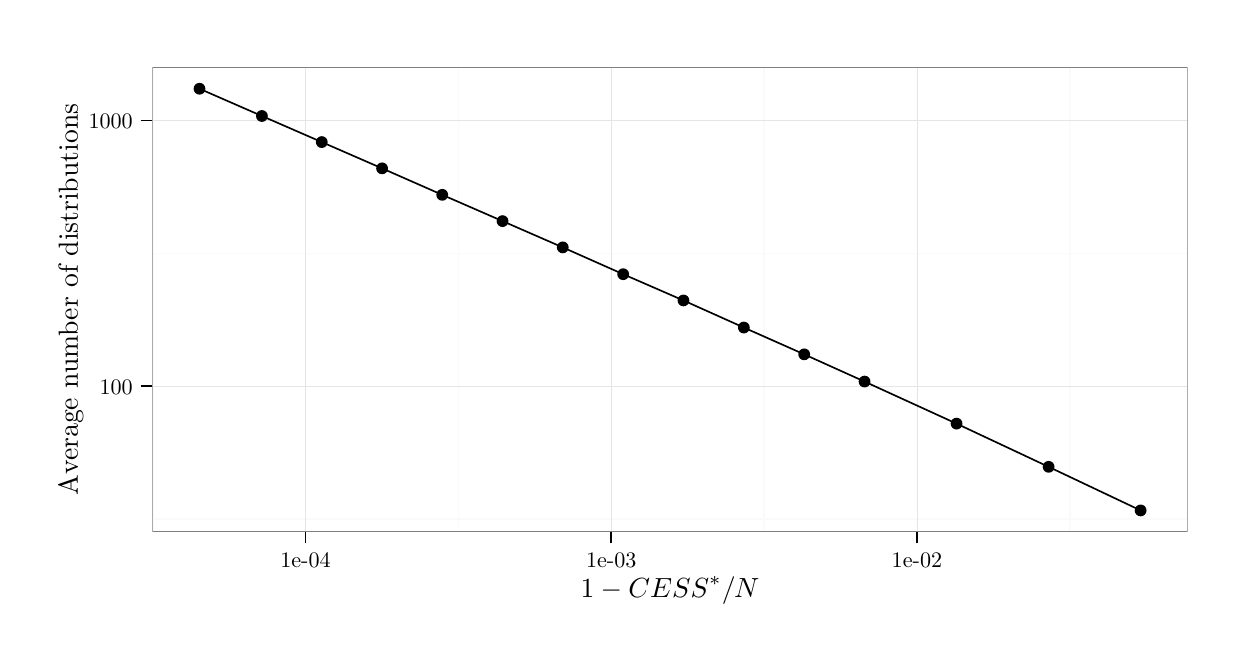
\begin{tikzpicture}[x=1pt,y=1pt]
\definecolor[named]{fillColor}{rgb}{1.00,1.00,1.00}
\path[use as bounding box,fill=fillColor,fill opacity=0.00] (0,0) rectangle (433.62,216.81);
\begin{scope}
\path[clip] (  0.00,  0.00) rectangle (433.62,216.81);
\definecolor[named]{drawColor}{rgb}{1.00,1.00,1.00}
\definecolor[named]{fillColor}{rgb}{1.00,1.00,1.00}

\path[draw=drawColor,line width= 0.6pt,line join=round,line cap=round,fill=fillColor] ( -0.00,  0.00) rectangle (433.62,216.81);
\end{scope}
\begin{scope}
\path[clip] ( 45.09, 34.74) rectangle (419.17,202.36);
\definecolor[named]{fillColor}{rgb}{1.00,1.00,1.00}

\path[fill=fillColor] ( 45.09, 34.74) rectangle (419.17,202.36);
\definecolor[named]{drawColor}{rgb}{0.98,0.98,0.98}

\path[draw=drawColor,line width= 0.6pt,line join=round] ( 45.09, 39.23) --
	(419.17, 39.23);

\path[draw=drawColor,line width= 0.6pt,line join=round] ( 45.09,135.22) --
	(419.17,135.22);

\path[draw=drawColor,line width= 0.6pt,line join=round] ( 45.17, 34.74) --
	( 45.17,202.36);

\path[draw=drawColor,line width= 0.6pt,line join=round] (155.64, 34.74) --
	(155.64,202.36);

\path[draw=drawColor,line width= 0.6pt,line join=round] (266.11, 34.74) --
	(266.11,202.36);

\path[draw=drawColor,line width= 0.6pt,line join=round] (376.58, 34.74) --
	(376.58,202.36);
\definecolor[named]{drawColor}{rgb}{0.90,0.90,0.90}

\path[draw=drawColor,line width= 0.2pt,line join=round] ( 45.09, 87.23) --
	(419.17, 87.23);

\path[draw=drawColor,line width= 0.2pt,line join=round] ( 45.09,183.22) --
	(419.17,183.22);

\path[draw=drawColor,line width= 0.2pt,line join=round] (100.40, 34.74) --
	(100.40,202.36);

\path[draw=drawColor,line width= 0.2pt,line join=round] (210.87, 34.74) --
	(210.87,202.36);

\path[draw=drawColor,line width= 0.2pt,line join=round] (321.34, 34.74) --
	(321.34,202.36);
\definecolor[named]{fillColor}{rgb}{0.00,0.00,0.00}

\path[fill=fillColor] ( 62.09,194.74) circle (  2.13);

\path[fill=fillColor] ( 84.64,184.89) circle (  2.13);

\path[fill=fillColor] (106.27,175.47) circle (  2.13);

\path[fill=fillColor] (128.07,165.97) circle (  2.13);

\path[fill=fillColor] (149.80,156.41) circle (  2.13);

\path[fill=fillColor] (171.59,146.91) circle (  2.13);

\path[fill=fillColor] (193.35,137.42) circle (  2.13);

\path[fill=fillColor] (215.18,127.73) circle (  2.13);

\path[fill=fillColor] (236.97,118.24) circle (  2.13);

\path[fill=fillColor] (258.79,108.45) circle (  2.13);

\path[fill=fillColor] (280.59, 98.77) circle (  2.13);

\path[fill=fillColor] (302.40, 88.93) circle (  2.13);

\path[fill=fillColor] (335.65, 73.73) circle (  2.13);

\path[fill=fillColor] (368.91, 58.12) circle (  2.13);

\path[fill=fillColor] (402.16, 42.36) circle (  2.13);
\definecolor[named]{drawColor}{rgb}{0.00,0.00,0.00}

\path[draw=drawColor,line width= 0.6pt,line join=round] ( 62.09,194.74) --
	( 84.64,184.89) --
	(106.27,175.47) --
	(128.07,165.97) --
	(149.80,156.41) --
	(171.59,146.91) --
	(193.35,137.42) --
	(215.18,127.73) --
	(236.97,118.24) --
	(258.79,108.45) --
	(280.59, 98.77) --
	(302.40, 88.93) --
	(335.65, 73.73) --
	(368.91, 58.12) --
	(402.16, 42.36);
\definecolor[named]{drawColor}{rgb}{0.50,0.50,0.50}

\path[draw=drawColor,line width= 0.6pt,line join=round,line cap=round] ( 45.09, 34.74) rectangle (419.17,202.36);
\end{scope}
\begin{scope}
\path[clip] (  0.00,  0.00) rectangle (433.62,216.81);
\definecolor[named]{drawColor}{rgb}{0.00,0.00,0.00}

\node[text=drawColor,anchor=base east,inner sep=0pt, outer sep=0pt, scale=  0.80] at ( 37.98, 84.30) {100};

\node[text=drawColor,anchor=base east,inner sep=0pt, outer sep=0pt, scale=  0.80] at ( 37.98,180.29) {1000};
\end{scope}
\begin{scope}
\path[clip] (  0.00,  0.00) rectangle (433.62,216.81);
\definecolor[named]{drawColor}{rgb}{0.00,0.00,0.00}

\path[draw=drawColor,line width= 0.6pt,line join=round] ( 40.82, 87.23) --
	( 45.09, 87.23);

\path[draw=drawColor,line width= 0.6pt,line join=round] ( 40.82,183.22) --
	( 45.09,183.22);
\end{scope}
\begin{scope}
\path[clip] (  0.00,  0.00) rectangle (433.62,216.81);
\definecolor[named]{drawColor}{rgb}{0.00,0.00,0.00}

\path[draw=drawColor,line width= 0.6pt,line join=round] (100.40, 30.47) --
	(100.40, 34.74);

\path[draw=drawColor,line width= 0.6pt,line join=round] (210.87, 30.47) --
	(210.87, 34.74);

\path[draw=drawColor,line width= 0.6pt,line join=round] (321.34, 30.47) --
	(321.34, 34.74);
\end{scope}
\begin{scope}
\path[clip] (  0.00,  0.00) rectangle (433.62,216.81);
\definecolor[named]{drawColor}{rgb}{0.00,0.00,0.00}

\node[text=drawColor,anchor=base,inner sep=0pt, outer sep=0pt, scale=  0.80] at (100.40, 21.77) {1e-04};

\node[text=drawColor,anchor=base,inner sep=0pt, outer sep=0pt, scale=  0.80] at (210.87, 21.77) {1e-03};

\node[text=drawColor,anchor=base,inner sep=0pt, outer sep=0pt, scale=  0.80] at (321.34, 21.77) {1e-02};
\end{scope}
\begin{scope}
\path[clip] (  0.00,  0.00) rectangle (433.62,216.81);
\definecolor[named]{drawColor}{rgb}{0.00,0.00,0.00}

\node[text=drawColor,anchor=base,inner sep=0pt, outer sep=0pt, scale=  1.00] at (232.13, 10.84) {$1 - \text{CESS}^*/N$};
\end{scope}
\begin{scope}
\path[clip] (  0.00,  0.00) rectangle (433.62,216.81);
\definecolor[named]{drawColor}{rgb}{0.00,0.00,0.00}

\node[text=drawColor,rotate= 90.00,anchor=base,inner sep=0pt, outer sep=0pt, scale=  1.00] at ( 18.16,118.55) {Average number of distributions};
\end{scope}
\end{tikzpicture}

\end{document}
